\documentclass[tikz,border=4pt]{standalone}
\usepackage{tikz}
\usetikzlibrary{shapes.geometric, arrows.meta, positioning}

\begin{document}
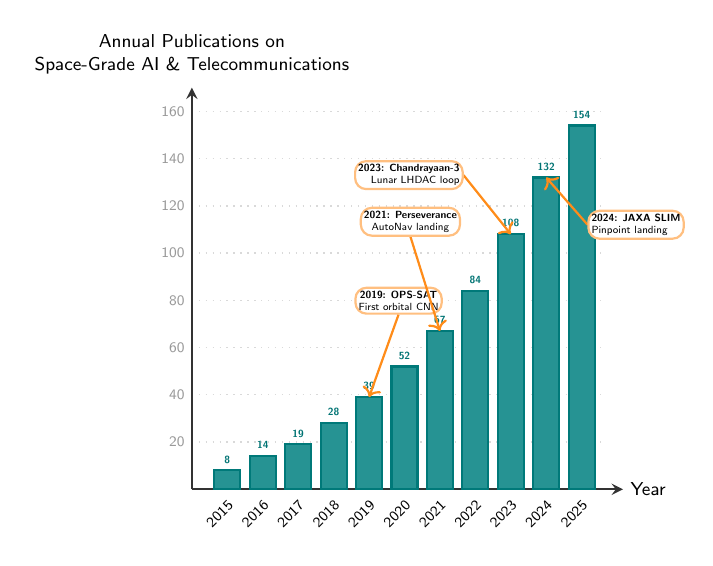
\begin{tikzpicture}[
    scale=0.75,
    transform shape,
    font=\sffamily\small,
    axis/.style={thick, ->, >=stealth, draw=black!80},
    barTeal/.style={fill=teal!85, draw=teal!95!black, thick},
    grid/.style={draw=gray!30, dotted, line width=0.5pt}
]
    % Grid lines (Y-axis grid)
    \foreach \y in {20, 40, 60, 80, 100, 120, 140, 160} {
        \draw [grid] (-0.5, \y*0.04) -- (6.5, \y*0.04);
        \node [left, font=\scriptsize\sffamily, text=gray!80] at (-0.5, \y*0.04) {\y};
    }
    
    % Axes
    \draw [axis] (-0.5, 0) -- (6.8, 0) node [right] {Year};
    \draw [axis] (-0.5, 0) -- (-0.5, 6.8) node [above, align=center, yshift=0.1cm] {Annual Publications on\\ Space-Grade AI \& Telecommunications};
    
    % Data bars (spaced 0.6cm apart)
    \foreach \x/\year/\count in {
        0.1/2015/8,
        0.7/2016/14,
        1.3/2017/19,
        1.9/2018/28,
        2.5/2019/39,
        3.1/2020/52,
        3.7/2021/67,
        4.3/2022/84,
        4.9/2023/108,
        5.5/2024/132,
        6.1/2025/154
    } {
        % Draw Bar
        \draw [barTeal] (\x-0.22, 0) rectangle (\x+0.22, \count*0.04);
        % Value above bar
        \node [above, font=\tiny\sffamily\bfseries, text=teal!90!black] at (\x, \count*0.04) {\count};
        % Year below axis
        \node [below, font=\scriptsize\sffamily, rotate=45, anchor=north east] at (\x, 0) {\year};
    }
    
    % Annotations for key mission milestones
    \draw [thick, <-, draw=orange!90] (2.5, 39*0.04) -- ++(0.5, 1.4) node [above, align=center, font=\tiny\sffamily, fill=white, draw=orange!50, rounded corners, inner sep=1.5pt] {\textbf{2019: OPS-SAT}\\First orbital CNN};
    
    \draw [thick, <-, draw=orange!90] (3.7, 67*0.04) -- ++(-0.5, 1.6) node [above, align=center, font=\tiny\sffamily, fill=white, draw=orange!50, rounded corners, inner sep=1.5pt] {\textbf{2021: Perseverance}\\AutoNav landing};
    
    \draw [thick, <-, draw=orange!90] (4.9, 108*0.04) -- ++(-0.8, 1.0) node [left, align=right, font=\tiny\sffamily, fill=white, draw=orange!50, rounded corners, inner sep=1.5pt] {\textbf{2023: Chandrayaan-3}\\Lunar LHDAC loop};
    
    \draw [thick, <-, draw=orange!90] (5.5, 132*0.04) -- ++(0.7, -0.8) node [right, align=left, font=\tiny\sffamily, fill=white, draw=orange!50, rounded corners, inner sep=1.5pt] {\textbf{2024: JAXA SLIM}\\Pinpoint landing};
    
\end{tikzpicture}
\end{document}
